% copyright (c) 2015 Synrc Research Center

\documentclass{svproc}
\usepackage{amscd}
\usepackage{listings}
\usepackage[numbers]{natbib}
\usepackage[only,llbracket,rrbracket,llparenthesis,rrparenthesis]{stmaryrd}
\usepackage{graphicx}
\usepackage{amsmath}
\usepackage{amssymb}
\usepackage{txfonts}
\usepackage[utf8]{inputenc}

\begin{document}

\title{Constructive Proof that Nat equals Fix Maybe}
\author{Maksym Sokhatskyi and Pavlo Maslianko}
\institute{National Technical University of Ukraine ``Igor Sikorsky Kyiv Polytechnical Institute''}

\maketitle

\section{Intro}

After formulating Type Theory for model quantifiers using Pi and Sigma types in 1972\cite{Lof72}
Per Martin-Lof added identity Equ types in 1984\cite{Lof84}. Later identity types was extended
to non-trivial structural higher equalities as was shown by Martin Hofmann
and Thomas Streicher in 1998\cite{Hofmann96}. However formal constructing of identity type
eliminators was made possible after introduction of Cubical Type Theory in 2017\cite{Mortberg17}.
CTT extends MLTT with interval I=[0,1] and its de Morgan algebra: 0, 1, r, min(r,s), max(r,s)
allowing constructive proofs of earlier models based on groupoid interpretation.

In this paper we want to present the constructive formulation of proof
that two values of different types are equal using constructive heterogenous equality.
At the end we will use both Path Isomorphism and Univalence for that purposes.
During story of comparing two zeros we will show minimal set of primitives needed
for performing this task in cubical type checker. Most of
them were imposible to derive in pure MLTT. We show these primitives in dependency order
while constructing our proof. They cover different topics in type theory, namely:

\begin{itemize}
\item Complete Formal Specification of MLTT
\item Contractability and Infinity Groupoids
\item Constructive J
\item Functional Extensionality
\item Fibers and Equivalence
\item Isomorphism
\item Nat = Fix Maybe
\end{itemize}

These primitives form a valuable part of
base library, so this arcticle could be considered as an brief introduction
to several modules: {\bf proto\_path}, {\bf proto\_equiv}, {\bf pi},
{\bf sigma}, {\bf mltt}, {\bf path}, {\bf iso}.

\begin{figure}[h]
  \centerline{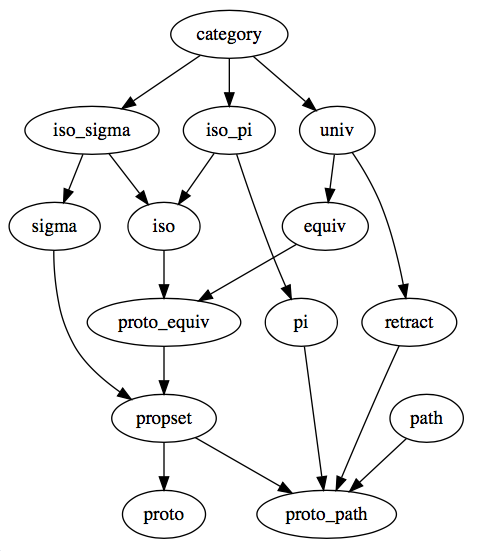
\includegraphics[scale=0.26]{baselib}}
  \caption{The Groupoid Infinity base library}
\end{figure}

\newpage
\section{MLTT Type Theory}

\subsection{Syntax Notes}

Types are the analogues of sets in ZFC, or objects in topos theory, or spaces in analisys.
Types contains elements, or points, or inhabitans and it's denoted $a : A$ and there
is definitional equality which usually built into type checker and compare normal forms.

\begin{equation}
\tag{terms and types}
a : A
\end{equation}

\begin{equation}
\tag{definitional equality}
x = [ y : A ]
\end{equation}

MLTT type theory with Pi and Sigma types was formulated using
natural deduction inference rules as a language.
The inference rules in that language will
be translated to cubicaltt in our article.

\begin{equation}
\tag{natural deduction}
\dfrac
{(A: U)\ (B: A \rightarrow U)}
{(x: A) \rightarrow B(x): U}
\end{equation}
\\
Equvalent definition in cubicaltt.

\begin{equation}
\tag{cubicaltt}
Pi\ (A: U)\ (B: A \rightarrow U): U = (x: A) \rightarrow B(x)
\end{equation}

The function name is an inference rule name,
everything from name to semicolon is context conditions,
and after semicolon is a new consruction derived from context conditions.
From semicolon to equality sign we have type and after
equ sign we have the term of that type.
If the types are treated as spaces then terms are points in these spaces.

According to MLTT each type has 4 sorts of inference rules:
Formation, Introduction, Eliminators and Computational rules.
Formation rules are formal definition of spaces while introduction rules
are methods how to create points in these spaces. Introduction rules increase term size,
while eliminators reduce term size. Computational rules always
formulated as equations that represents reduction rules,
or operational semantics.

\subsection{Pi types}

Pi types represent spaces of dependent functions.
With Pi type we have one lambda constructor
and one application eliminator. When $B$ is not dependent on $x:A$
the Pi is just a non-dependent total function $A \rightarrow B$.
Pi has one lambda function constructor, and its eliminator, the application.

$$Pi(A,B) = \prod_{x:A} B(x) : U,\ \ \ 
  \lambda x . b : \prod_{x:A} B(x)$$

$$\prod_{f:\prod_{x:A}B(x)}\prod_{a:A} f a : B (a)$$

\begin{lstlisting}[mathescape=true]
Pi (A:U) (B:A->U) : U = (x:A)->B(x)
lambda (A:U) (B:A->U) (a:A) (b:B(a)): A->B(a) = \(x:A)->b
app (A:U) (B:A->U) (a:A) (f:A->B(a)): B(a) = f(a)
\end{lstlisting}

\subsection{Sigma types}

Sigma types represents a dependent cartesian products.
With sigma type we have pair constructor and two eliminators,
its first and second projections. When $B$ is not dependent on $x:A$
the Sigma is just a non-dependent product $A \times B$.
Sigma has one pair constructor and two eliminators, its projections.

$$Sigma(A,B) = \sum_{x:A} B(x) : U,\ \ \ 
  (a,b) : \sum_{x:A} B(x)$$

$$\pi_1 : \prod_{f:\sum_{x:A}B(x)}A\ ,\ \ \ \pi_2 : \prod_{f:\sum_{x:A}B(x)}B(\pi_1(f))$$

As Pi and Sigma are dual the Sigma type could be formulated
in terms of Pi type using Church encoding, thus Sigma is optional.
The type systems which contains only Pi types called Pure or PTS.

\begin{lstlisting}[mathescape=true]
Sigma (A:U) (B:A->U): U = (x:A) * B(x)
pair (A:U) (B:A->U) (a: A) (b: B(a)): Sigma A B = (a,b)
pr1 (A:U) (B:A->U) (x: Sigma A B): A = x.1
pr2 (A:U) (B:A->U) (x: Sigma A B): B (pr1 A B x) = x.2
\end{lstlisting}

\newpage
\subsection{Equ types}

For modeling propositional equality later in 1984 was introduced Equ type.
However unlike Pi and Sigma the eliminator J of Equ type is not derivanle in MLTT.

$$Equ(x,y) = \prod_{x,y:A} x =_A y : U,\ \ \ 
  reflect : \prod_{a:A} a =_A a$$
$$D : \prod_{x,y:A}^{A:U_i} x =_A y \rightarrow U_{i+1},\ \ \ 
  J : \prod_{C: D} \prod_{x:A} C(x,x,reflect(x)) \rightarrow \prod_{y:A} \prod_{p:x=_A y} C(x,y,p)$$

Eliminator of Equality has complex form and underivable in MLTT.

\begin{lstlisting}[mathescape=true]
Equ       (A: U) (x y: A): U = undefined
reflect   (A: U) (a: A): Equ A a a = undefined
D         (A: U) : U = (x y: A) -> Equ A x y -> U
J         (A: U) (x y: A) (C: D A) (d: C x x (reflect A x))
          (p: Equ A x y): C x y p = undefined
\end{lstlisting}

Starting from MLTT until cubicaltt there was no computational semantics
for J rules and in Agda and Coq it was formulated using inductive data types
wrapper around built-in primitives (J) in the core:

\begin{lstlisting}[mathescape=true]
data Equality (A:U) (x y:A) = refl_ (_: Equ A x y)
reflection (A:U) (a:A): Equality A a a = refl_ (reflect A a)
\end{lstlisting}

Heterogenous equality is needed for computational rule of Equ type.
And also this is crucial to our main task, constructive
comparison of two values of different types. We leave the definition blank
until introdure cubical primitives, here is just MLTT signature of HeteroEqu
which is undervable in MLTT.

\begin{lstlisting}[mathescape=true]
HeteroEqu (A B: U) (a: A) (b: B) (P: Equ U A B) : U = undefined
\end{lstlisting}

\newpage
\subsection{Complete Formal Specification of MLTT}

MLTT needn't and hasn't the underlying logic, the Logical Framework could be constructed directly in MLTT.
According to Brouwer-Heyting-Kolmogorov interpretation the propositions are types,
Pi is an universal quantifier, Sigma is existential quantifier.
Implication is given by Pi over types, conjunction is cartesian
product of tpes and disjunction is disjoint sum of types.

So we can build LF for MLTT inside MLTT. Specification could be formulated as a
single Sigma chain holding the computation system and its theorems in one package.
Carrying object along with its properties called type refinement, so this type
represents a refined MLTT:

\begin{lstlisting}[mathescape=true]
MLTT (A:U): U
  = (Pi_Former:  (A->U)->U)
  * (Pi_Intro:   (B:A->U) (a:A)->B a->(A->B a))
  * (Pi_Elim:    (B:A->U) (a:A)->(A->B a)->B a)
  * (Pi_Comp1:   (B:A->U) (a:A) (f:A->B a) -> Equ (B a)
                 (Pi_Elim B a (Pi_Intro B a (f a)))(f a))
  * (Pi_Comp2:   (B: A->U) (a:A) (f:A->B a) ->
                 Equ (A->B a) f (\(x:A)->Pi_Elim B a f))
  * (Sig_Former: (A->U)->U)
  * (Sig_Intro:  (B:A->U) (a:A)->(b:B a)->Sigma A B)
  * (Sig_Elim1:  (B:A->U)->(_: Sigma A B)->A)
  * (Sig_Elim2:  (B:A->U)->(x: Sigma A B)->B (pr1 A B x))
  * (Sig_Comp1:  (B:A->U) (a:A) (b: B a)->Equ A a
                 (Sigma_Elim1 B (Sigma_Intro B a b)))
  * (Sig_Comp2:  (B:A->U) (a:A) (b:B a)->Equ (B a) b
                 (Sigma_Elim2 B (a,b)))
  * (Id_Former:  A->A->U)
  * (Id_Intro:   (a:A) -> Equ A a a)
  * (Id_Elim:    (a x: A) (C: predicate A a)
                 (d:C a(Id_Intro a))(p:Equ A a x)->C x p)
  * (Id_Comp:    (x y:A)(C: D A)(p: Equ A x y) (b: C x x (reflect A x))
                 (X: Equ U (C x x (reflect A x)) (C x y p)) ->
                 HeteroEqu X b (J A x C b y p)) * Unit
\end{lstlisting}

Even more complex challanges on Equ type was introduced such
as heterogenous equality $HeteroEqu$ needed to formulation
of computational rule $Id\_Comp$ of $Equ$ type. Presheaf model of Type Theory, specifically
Cubical Sets with interval $[0,1]$ and
its algebra was introduced to solve derivability issues. So the instance of MLTT is packed
with all the type inference rules along with operational semantics:

\begin{lstlisting}[mathescape=true]
instance (A: U): MLTT A
    = (Pi A, lambda A, app A, comp1 A, comp2 A,
       Sigma A, pair A, pr1 A, pr2 A, comp3 A, comp4 A,
       Equ A, reflect A, J A, comp5 A, tt)
\end{lstlisting}

\newpage
\section{Path interval operations}

The path equality is modeled as an interval [0,1] with
its de Morgan algebra 0, 1, r, min(r,s), max(r,s). According to underlying theory
it has lambdas, application, composition and gluening of [0,1] interval and Min and Max
functions over interval arguments. This is enought to formulate and prove path
isomorphism and heterogenous equality.

\begin{lstlisting}[mathescape=true]
Heterogenous Path: (p: Path U A B) -> PathP p A B
Function over [0,1]: `<i> A`.
Application of Path to [0,1]: `<i> p @ i`
Path Composition: `comp (Path A a b) x []`.
Path Gluening: `Glue A B [] -> Path U A B`
Min: `<i j> p @ i /\ j)`.
Max: `<i j> p @ i \/ j)`.
\end{lstlisting}

\begin{lstlisting}[mathescape=true]
composition (A : U) (a b c : A) (p : Path A a b)
    (q : Path A b c) : Path A a c
    = <i> comp (<j>A) (p @ i) [ (i=1) -> q,
                                (i=0) -> <j> a ]
\end{lstlisting}

\section{Contractability and Higher Equalities}

A type $A$ is contractible, or a singleton, if there is $a : A$,
called the center of contraction, such that $a = x$ for all $x : A$:
A type $A$ is proposition if any x,y: A are equals.
A type is a Set if all equalities in A form a prop.
It is defined as recursive definition.

$$isContr = \sum_{a:A}\prod_{x:A} a =_A x,\ \ 
  isProp(A) = \prod_{x,y:A} x =_A y,\ \ 
  isSet = \prod_{x,y:A} isProp\ (x =_A y),\ \ $$
$$isGroupoid = \prod_{x,y:A} isSet\ (x =_A y),\ \ 
  PROP = \sum_{X:U}isProp(X),\ \ 
  SET = \sum_{X:U}isSet(X),...$$

The following types are inhabited: isSet PROP, isGroupoid SET.
All these functions are defined in {\bf propset} module.

\begin{lstlisting}[mathescape=true]
data N = Z | S (n: N)
n_grpd (A: U) (n: N): U = (a b: A) -> ((rec A a b) n) where
  rec (A: U) (a b: A): (k: N) -> U = split
    Z -> Path A a b
    S n -> n_grpd (Path A a b) n

isContr (A: U): U = (x:A) * ((y: A) -> Equ A x y)
isProp      (A: U): U = n_grpd A Z
isSet       (A: U): U = n_grpd A (S Z)
isGroupoid  (A: U): U = n_grpd A (S (S Z))
PROP      : U = (X:U) * isProp X
SET       : U = (X:U) * isSet  X
GRPOUPOID : U = (X:U) * isGroupoid X
\end{lstlisting}

\newpage
\section{Constructive J}

The very basic ground of type checker is heterogenous equality $PathP$ and contructive
implementation of reflection rule as lambda over interval $[0,1]$ that
return constant value $a$ on all domain.

\begin{lstlisting}[mathescape=true]
Path (A:U) (a b: A): U = PathP (<i> A) a b
HeteroEqu (A B: U) (a: A) (b: B) (P: Equ U A B) : U = Path P a b
refl (A:U) (a: A): Path A a a = <i> a
\end{lstlisting}

$$trans : \prod_{p:A=_U B}^{A,B:U} \prod_{a:A} B,\ \ \ singleton : \prod_{x:A}^{A:U} \sum_{y:A} x =_A y $$

$$subst : \prod_{a,b:A}^{A:U,B:A\rightarrow U} \prod_{p: a =_A b} \prod_{e:B(a)} B(b), \ \ \ 
  congruence : \prod_{f:A\rightarrow B}^{A,B:U} \prod_{a,b:A} \prod_{p:a =_A b} f(a) =_B f(b) $$

Transport tranfers the element of type to another by given path equality of the types.
Substitution is like transport but for dependent functions values: by given dependent function
and path equality of points in the function domain we can replace the value of dependent function
in one point with value in the second point. Congruence states that for a given function
and for any two points in the function domain, that are connected, we can state that function
values in that points are equal.

\begin{lstlisting}[mathescape=true]
singl (A:U) (a:A): U = (x: A) * Path A a x
trans (A B:U) (p: Path U A B) (a: A): B = comp p a []
congruence (A B: U) (f:A->B) (a b: A)
           (p: Path A a b): Path B (f a) (f b)
           = <i> f (p @ i)

subst (A:U) (P:A->U) (a b: A)
      (p: Path A a b) (e: P a): P b
      = trans (P a) (P b) (congruence A U P a b p) e

contrSingl (A : U) (a b : A) (p : Path A a b):
           Path (singl A a) (a,refl A a) (b,p)
           = <i> (p @ i, <j> p @ i /\ j )
\end{lstlisting}

Then we can derive J using $contrSingl$ and $subst$:

\begin{lstlisting}[mathescape=true]
J (A : U) (x y: A) (C: D A)
  (d : C x x (refl A x)) (p: Path A x y) : C x y p =
    subst (singl A x) T (x, refl A x) (y, p)
    (contrSingl A x y p) d where T (z : singl A x) : U
    = C (z.1) (z.2)
\end{lstlisting}

These function are defined in {\bf proto\_path} module, and all of them
except singleton definition are underivable in MLTT.

\section{Functional Extensionality}

Function extensionality is another example of underivable theorems in MLTT, it
states if two functions with the same type and they always equals for
any point from domain, we can prove that these function are equal.
We distinguish dependent and non-dependent versions by signature,
however proof term is the same in both cases.

$$funExtDependent: \prod_{[f,g: (x:A) \rightarrow B(x)]}^{A: U,B:A\rightarrow U}\prod_{[x:A,p:A\rightarrow f(x) =_{B(x)} g(x)]} f =_{A\rightarrow B(x)} g$$

\begin{lstlisting}[mathescape=true]
funExtDependent  (A: U) (B: A -> U)
       (f g: (x : A) -> B x)
       (p : (x : A) -> Path (B x) (f x) (g x)) :
       Path ((y : A) -> B y) f g = <i> \(a : A) -> (p a) @ i

funExt (A B: U) (f g: A -> B)
       (p: (x : A) -> Path B (f x) (g x)):
       Path (A -> B) f g = <i> \(a : A) -> p a @ i
\end{lstlisting}

\section{Fibers and Equivalence}

The fiber of a map $f : A \rightarrow B$ over a point $y : B$ is family over x
of Sigma pair containing the point $x$ and proof that $f(x)=_B y$.

$$fiber : \prod_{f:A->B}^{A,B:U}\prod_{x:A,y:B}\sum f(x) =_B y,\ \ \ 
  isEquiv : \prod_{f:A->B}^{A,B:U}\prod_{y:B} isContr(fiber(f,y))$$
$$equiv : \sum_{f:A->B}^{A,B:U} isEquiv(f) \ \ \ 
  pathToEquiv: \prod_{p: X =_U Y}^{X,Y:U} equiv_U(X,Y)$$.

Contractability of fibers called isEquiv predicate. The Sigma pair of
a function and that predicate called equivalence, or equiv. Now we
can prove that singletons are contractible and write a conversion
function $X=_U Y \rightarrow equiv(X,Y)$.

\begin{lstlisting}[mathescape=true]
fiber   (A B: U) (f: A -> B) (y: B): U = (x: A) * Path B y (f x)
isEquiv (A B: U) (f: A -> B): U = (y: B) -> isContr (fiber A B f y)
equiv   (A B: U): U = (f: A -> B) * isEquiv A B f

singletonIsContractible (A:U) (a:A): isContr (singl A a)
    = ((a,refl A a), \ (z:(x:A) * Path A a x) ->
    contrSingl A a z.1 z.2)

pathToEquiv (A X : U) (p : Path U X A) : equiv X A
    = subst U (equiv A) A X p (idEquiv A)
\end{lstlisting}

\section{Isomorphism}

The general idea to build path between values of different type is first
to build isomorphism between types, defined as decode and encode functions (f and g),
such that $f \circ g = id, g \circ f = id$.

$$Iso(A,B) = \sum_{[f:A\rightarrow B]}\sum_{[g:B\rightarrow A]}\Biggl( \prod_{x:A} [ g(f(x)) =_A x ] \times \prod_{y:B} [ f(g(y) =_B y ] \Biggr)$$

$$isoToEquiv(A,B) : Iso(A,B) \rightarrow Equiv(A,B)$$
$$isoToPath(A,B) : Iso(A,B) \rightarrow A =_U B$$

$lemIso$ proof is a bit longread, you may refer to Github
repository\footnote{http://github.com/groupois/infinity/tree/master/priv/iso.ctt}.
The by proof of $isoToEquiv$ using $lemIso$ we define $isoToPath$ as
Glue of A and B types, providing $equiv(A,B)$. Glue operation first appear in
proving transprt values of different type across their path equalities which are being constructed
using encode and decode functions that represent isomorphism. Also Glue operation
appears in constructive implementation of Univalence axiom\cite{Mortberg17}.

\begin{lstlisting}[mathescape=true]
lemIso  (A B : U) (f: A->B) (g:B->A)
        (s: (y:B) -> Path B (f(g(y)))y)
        (t: (x:A) -> Path A (g(f(x)))x) (y:B) (x0 x1:A)
        (p0: Path B y (f(x0))) (p1: Path B y (f(x1))):
        Path (fiber A B f y) (x0,p0) (x1,p1) = undefined

isoToEquiv (A B: U) (f: A -> B) (g: B -> A)
        (s: (y: B) -> Path B (f (g y)) y)
        (t: (x: A) -> Path A (g (f x)) x): isEquiv A B f =
  \(y:B) -> ((g y,<i>s y@-i),\ (z:fiber A B f y) ->
    lemIso A B f g s t y (g y) z.1 (<i>s y@-i) z.2)

isoToPath (A B:U) (f:A->B)(g:B->A)
        (s: (y:B)->Path B (f(g(y)))y)
        (t: (x:A)->Path A (g(f(x)))x): Path U A B =
        <i> Glue B [(i=0)->(A,f,isoToEquiv A B f g s t),
                    (i=1)->(B,idfun B,idIsEquiv B) ]
\end{lstlisting}

\newpage
\section{Nat = Fix Maybe}

\begin{lstlisting}[mathescape=true]
natToMaybe: nat -> fix maybe = split
  zero -> Fix nothing
  suc n -> Fix (just (natToMaybe n))

maybeToNat : fix maybe -> nat = split
  Fix m -> split nothing -> zero
                 just f -> suc (maybeToNat f)

natMaybeIso: (a: nat) ->
    Path nat (maybeToNat (natToMaybe a)) a = split
         zero -> <i> zero
         suc n -> <i> suc (natMaybeIso n @ i)

maybeNatIso : (a : fix maybe) ->
    Path (fix maybe) (natToMaybe (maybeToNat a)) a = split
         Fix m -> split nothing -> <i> Fix nothing
                        just f -> <i> Fix (just (maybeNatIso f @ i))

maybenat_ : Path U (fix maybe) nat
    = isoPath (fix maybe) nat
              maybeToNat natToMaybe
              natMaybeIso maybeNatIso

> PathElem nat2 nat zero2 zero nat2nat
EVAL: PathP (<!0> Glue nat [ (!0 = 0) -> (nat2,(toNat,(\(y : B)
-> ((g y,&lt;i&gt; (s y) @ -i),\(z : fiber A B f y) -> lemIso A B f g
s t y (g y) z.1 (&lt;i&gt; (s y) @ -i) z.2)) (A = nat2, B = nat, f =
toNat, g = fromNat, s = fromNatK, t = toNatK))), (!0 = 1) ->
(nat,((\(a : A) -> a) (A = nat),(\(a : A) -> ((a,refl A a),\(z:
fiber A A (idfun A) a) -> contrSingl A a z.1 z.2)) (A = nat)))])
zero2 zero
\end{lstlisting}

\section{Conclusion}
As you can see EXE language has enough expressive power to be used for
drawing MLTT axioms in computer science articles and papers.

\newpage

\bibliographystyle{aipnum-cp}
\bibliography{identity}

\end{document}
